The data yields and background estimation for all 84 search bins are shown in Fig~\ref{fig:84sbunblind}. No statistically significant excess in the data above the expectation from the standard model is observed. The \ttbar, $W$+jets and single top events are the largest source of the background. The $Z$+jets events can be dominant in the high \MET search bins. The QCD and rare backgrounds are small in all search bins. 

\begin{figure}[htbp]
 \begin{center}
  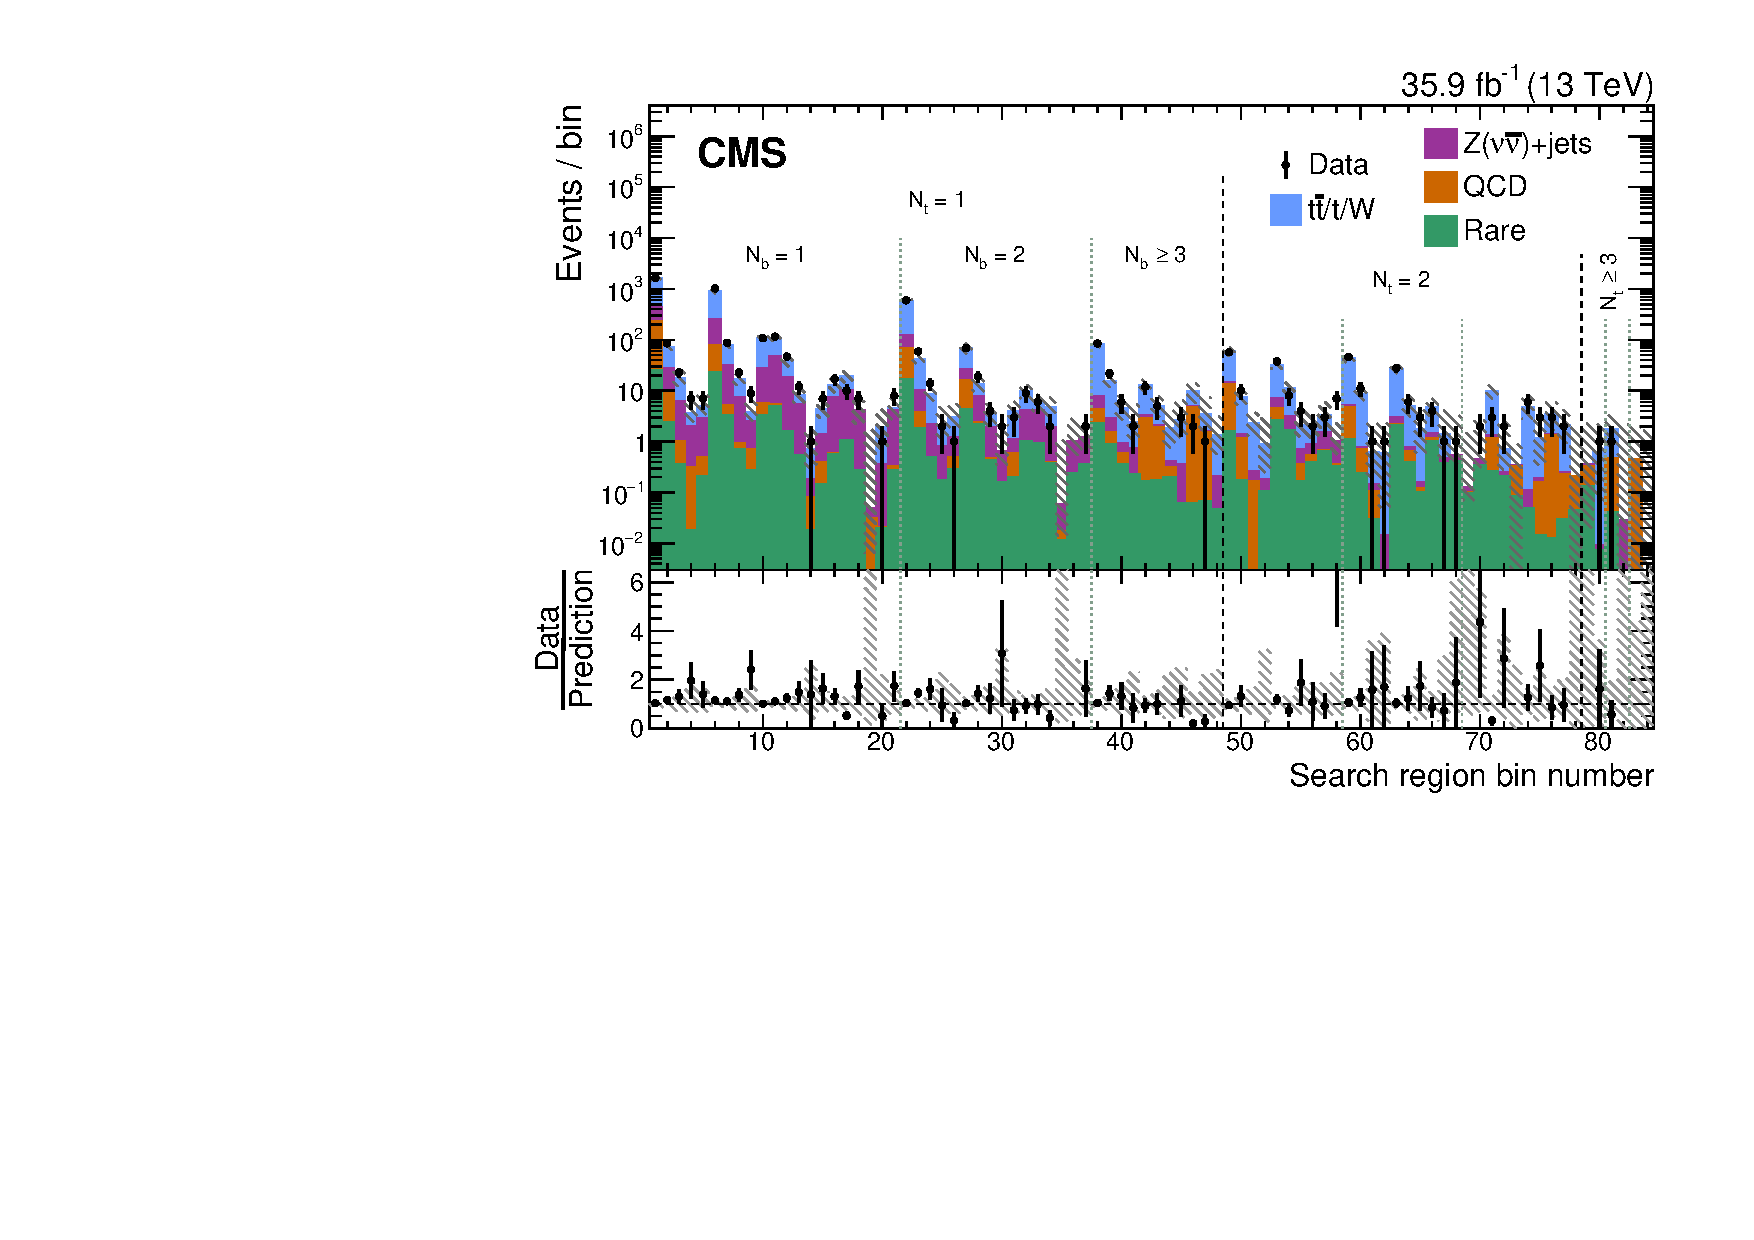
\includegraphics[width=0.8\textwidth]{sections/mc4/Results/figures/UnblindPlots.pdf}
 \end{center}
 \caption{Observed event yields in data (black points) and predicted SM background (filled solid area) for the 84 search bins. The lower panel shows the ratio of data over total background prediction in each search bin. For both panels, the error bars show the statistical uncertainty associated with the observed data counts, and the grey (blue) hatched bands indicate the statistical (systematic) uncertainties in the total predicted background.}
 \label{fig:84sbunblind}
\end{figure}

The analysis is interpreted as the upper limit of the signal model cross section. The upper limit of the signal model cross sections with 95\% confidence level are calculated, using a modified frequentist ($CL_{s}$) approach\cite{Cowan:2010js}. The $CL_{s}$ is defined in Eq~\ref{eq:c4cls}:

\begin{equation}
 \begin{aligned}
  CL_{s}=\frac{CL_{s+b}}{CL_{b}},
 \end{aligned}
 \label{eq:c4cls}
\end{equation}
where the $CL_{s+b}$ is the confidence level in signal plus background hypothesis, and $CL_{b}$ is the confidence level with the background only assumption. 

In the $CL_{s+b}$ calculation, we assume that the observed number of events n to follows a Poisson distribution with an expected value $E[n]=\mu s+b$. The s term is the mean number of events from a signal model, which is a known number from simulation. The b term is the expected number of background events, also a known number. The $\mu$ term is the signal acceptance, which is the value we need to obtain with likelihood. 

The b term is the expected number of background events from all sources. We treat the backgrounds as nuisance parameters, whose values are constrained by the control samples (e.g., the single muon control sample for the lost lepton and hadronic tau background, the inverted $\Delta \phi$ control sample for the QCD background, etc.). The control samples are defined as a Poisson distribution with mean value $E[n]=\tau b$. The $\tau$ term is a scale factor between the control sample region and signal region, for example, the translation factors in the QCD case. Therefore the likelihood function for $\mu$ and b can be expressed as Eq~\ref{eq:c4clslikelihood}:

\begin{equation}
 \begin{aligned}
	 L(\mu,b)= \prod_{i=1}^{N} \frac{(\mu s_{i}+\sum_{j=1}^{M}b_{ij})^{n_{i}}}{n_{i}!}e^{-(\mu s_{i}+\sum_{j=1}^{M}b_{ij})},
 \end{aligned}
 \label{eq:c4clslikelihood}
\end{equation}
where M is the number of different background categories. In this analysis, M=4: one category for the lost lepton and hadronic tau lepton background, and the other three for the Z+jets, QCD, and TTZ/rare backgrounds. N is the total number of search bins, $N=84$ in this analysis. Wilks's theorem\cite{Wilks:1938dza} states that the log of $CL_{s}$ is asymptotically $\chi^{2}$ distributed. This asymptotic method is applied in the limit setting to accelerate the process. The likelihood ratio is maximized following the procedure described in Ref~\cite{Cowan:2010js}.

We consider the following uncertainties in the signal yields: 

\begin{itemize}
\item {\bf MC statistics:} The statistical uncertainties in MC signal samples.
\item {\bf Luminosity:} A 2.6\% flat contribution is assigned.
\item {\bf lepton veto:} Lepton vetoes are categorized as the muon and electron vetoes, the muon and electron track vetoes and the pion track veto.
The numbers of signal events vetoed by each of the categories are evaluated. Then the yields are varied by the corresponding veto category uncertainties and propagated to be relative changes to the signal yields in the search bins. Here the amount of vetoed events effectively reflects the various lepton selection efficiencies.
The efficiency uncertainties in the lepton selections either come from the lepton scale factor group (for the muon and electron efficiencies) or dedicated studies by either the lost lepton (for the muon and electron track efficiencies) or the hadronic tau method (for the pion track efficiencies). The scale factors from lepton scale factor group are used in this thesis.
\item {\bf b-tag efficiency:} The b-tagging and mistagging scale factor uncertainties are applied as a function of the jet $p_{T}$ and $\eta$.
\item {\bf b-tag FastSim corrections:} The b-tagging and mistagging performance as derived from the fast simulation is corrected to match the
full simulation predictions. Separate correction factors are derived for b-jets, c-jets, and light-flavor-jets, as a function of the jet $p_{T}$ and $\eta$. As with the scale factors above, the correction factors for each type of jet are varied independently within their uncertainties and propagated to the signal bins. The correction factors and uncertainties are derived from an average mixture of \ttbar and signal events.
\item {\bf Trigger efficiency:} The signal samples are corrected for the trigger inefficiencies. The effect of trigger efficiency uncertainties on the signal samples is at most 2.6\% in the lowest \MET bins.
\item {\bf Pileup acceptance:}
The signal acceptance was found not to depend strongly on pileup, and an uncertainty is assigned to quantify this. The relative signal acceptance as a function of $n_{\text{vtx}}$ is modeled from Monte Carlo, and is applied to the normalized $n_{\text{vtx}}$ distribution in data.
The relative signal acceptance is modeled as a linear fit in two bins, $n_{\text{vtx}} < 20$ (low PU) or $n_{\text{vtx}} \geq 20$ (high PU). A confidence band for the linear fit is derived from the uncertainty in the relative acceptance due to the statistical uncertainty in the Monte Carlo event counts. The pileup acceptance uncertainty is found by calculating the expectation
value:
\begin{equation}
c = \sum_{n_{\text{vtx}}=0}^{100} f_{\text{MC}}(n_{\text{vtx}})g_{\text{data}}(n_{\text{vtx}}) \label{eq:puacc-expval},
\end{equation}
where $f_{\text{MC}}$ is taken from the central fit value or the lower or upper limit from the confidence band.
The $g_{\text{data}}(n_{\text{vtx}})$ term is measured in a single electron control region (requiring $\njets\geq2$, $n_{\text{electron}}=1$, and \texttt{HLT\_Elea27\_WPTight}).
The up and down variations of c are normalized to the value from the central variation of the fit. The magnitude of the uncertainty is found to be 0.2-4.1\%
\item {\bf Renormalization and factorization scales:} The uncertainty is calculated using the envelope of the weights obtained by varying the renormalization and factorization scales, $\mu_{R}$ and $\mu_{F}$, by factor of two \cite{Cacciari:2003fi,Catani:2003zt}. The effects on the signal shapes are considered as their uncertainties on the signal cross sections. %The effect on the T2tt signal samples ranges from 0 to 2.9\%.
\item {\bf ISR:} The ISR correction is applied and its uncertainty is propagated following the recommended procedure for Moriond 2017.
\item {\bf Jet Energy Corrections:} The jet energy corrections (JEC) are varied within the $p_{T}$ and $\eta$-dependent jet energy scale uncertainties available in the official database. A different set of corrections and uncertainties is used in fast simulation samples. These variations are propagated into the jet-dependent search variables, such as: \nbjets, \ntops, \MET, \MTTwo, \HT, $\Delta\phi(\MET,j_{i})$.
\item {\bf \MET uncertainty:} To account for uncertainties in \MET in the fast simulation, the evaluation of the signal yield is repeated using generator \MET. The average of both yields is used as an uncertainty.
\item {\bf PDFs:} The LHC4PDF\cite{Butterworth:2015oua} prescription for the uncertainty in the total cross section is included as $\pm$1 sigma band in the limit plots. As recommended by the SUSY group, no additional PDF uncertainty is included.
\item {\bf Full/FastSim scale for top quark reconstruction:} We use the full simulation to fastsim scale factor as measured in Ref~\cite{AN-16-461}. In the fastsim signal events for any of the reconstructed top quark candidates that are matched to a generator-level top quark, we apply the corresponding scale factor measured as a function of top quark $p_{T}$. We then propagate the statistical uncertainties on the scale factor to the signal yields in our search bins.
\item {\bf Top tagger data/MC difference:} As discussed in Ref~\cite{AN-16-461}, the top tagger efficiency agrees well between data and MC (full simulation) within uncertainties. We apply the measured correction factors for each type of the mono-jet, di-jet and tri-jet reconstructed top quark candidates. We then propagate the measured uncertainties to the signal yields in our search bins.
\end{itemize}

The analysis interpretations are presented in Fig~\ref{fig:signal_results}. The T2tt interpretation is not given for $|m_{\sTop}-m_{\chiOneZero}-m{t}|<25~GeV$ and $m_{\sTop}<275~GeV$ because the signal acceptance is difficult to model in these regions, due to the similarity between signal events and the standard model \ttbar events in these regions. 

The T5tttt interpretation is not presented for $m_{\chiOneZero}<50~GeV$ because of contamination from SM \ttbar events with fake \MET.
The solid black curves represent the observed exclusion contour with respect to NLO+NLL signal cross sections and the change in this contour due to variation of these cross sections within their theoretical uncertainties\cite{Borschensky:2014cia}. The dashed red curves indicate the mean expected exclusion contour and the region containing 68\% of the distribution of expected exclusion limits under the background-only hypothesis. 

\begin{figure}[ht!]
 \begin{centering}
  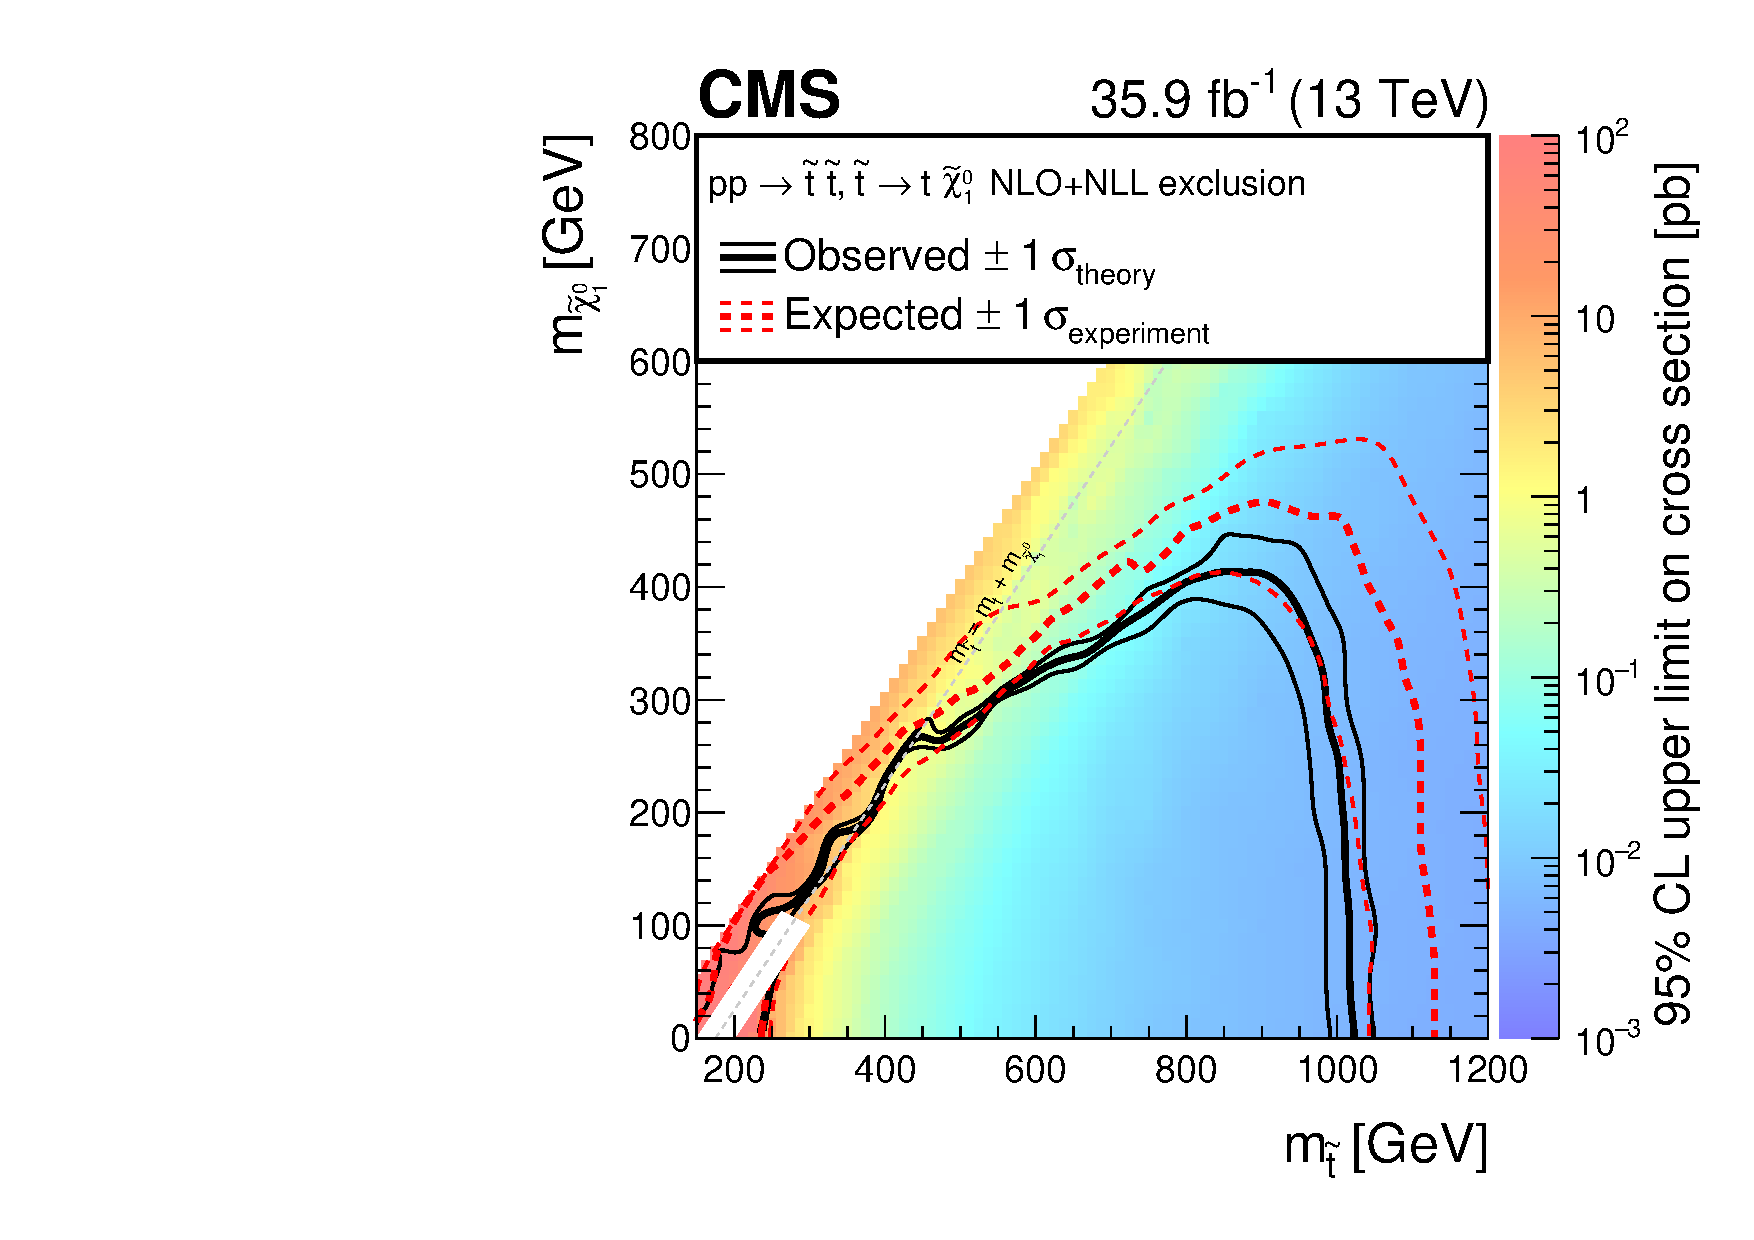
\includegraphics[width=0.50\textwidth]{sections/mc4/Results/figures/Covered_T2tt_OnlyXSEC.pdf}\\
  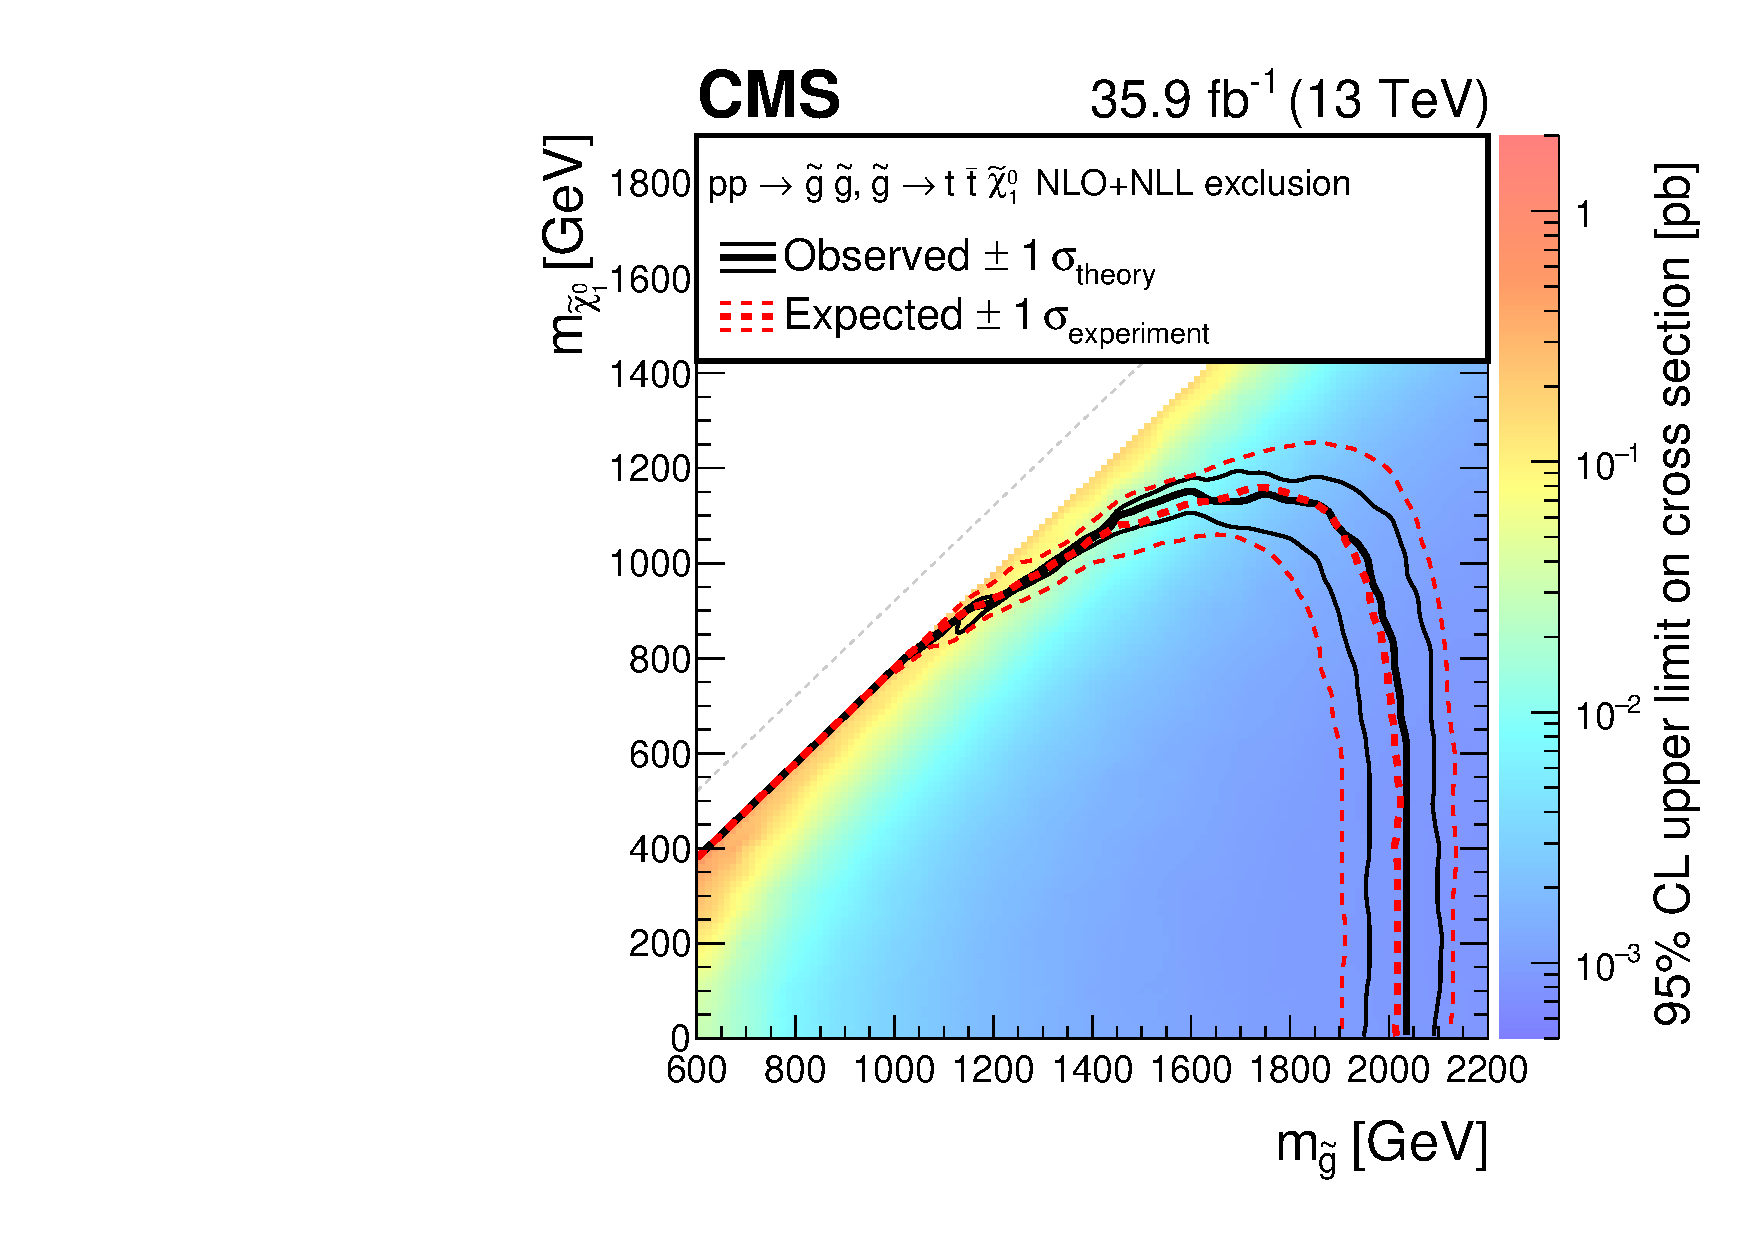
\includegraphics[width=0.40\textwidth]{sections/mc4/Results/figures/T1tttt_OnlyXSEC.pdf}
  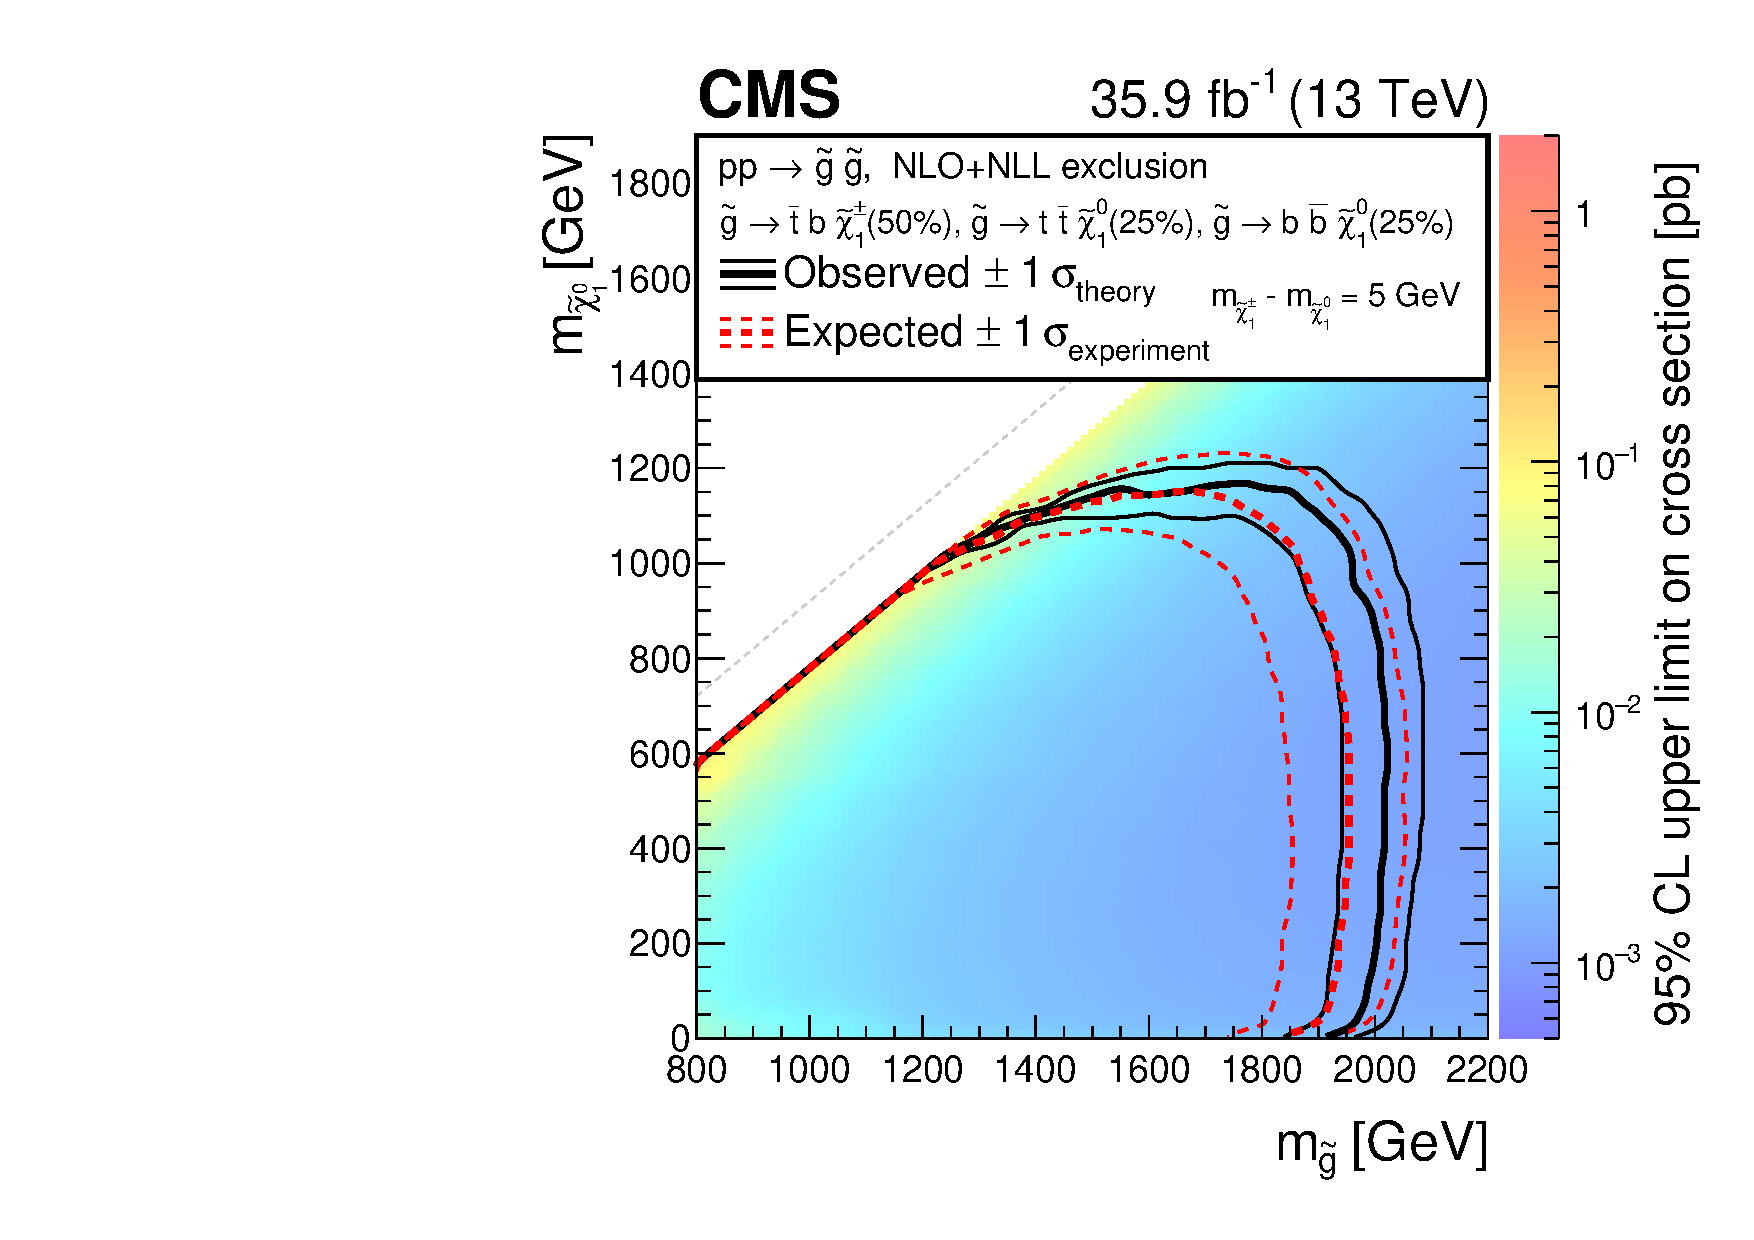
\includegraphics[width=0.40\textwidth]{sections/mc4/Results/figures/T1ttbb_OnlyXSEC.pdf}\\
  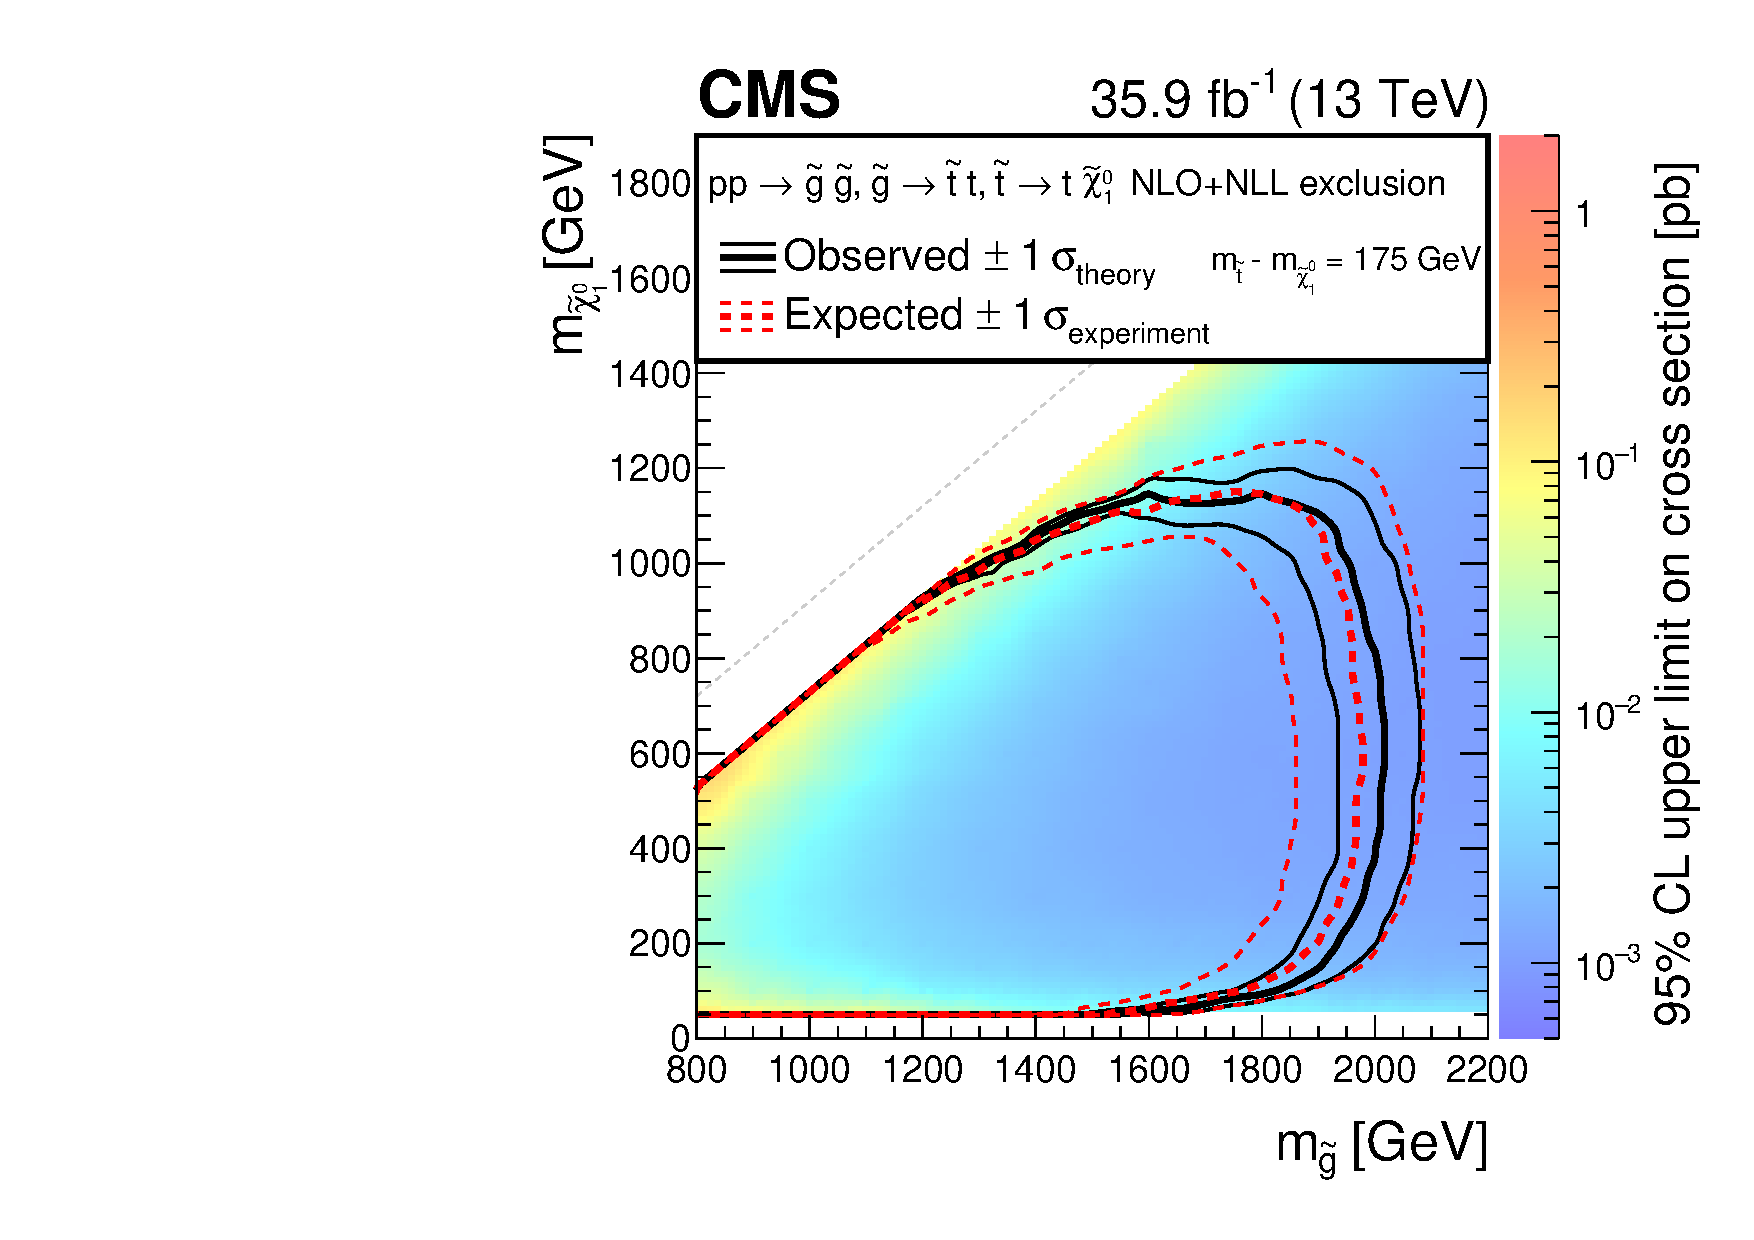
\includegraphics[width=0.40\textwidth]{sections/mc4/Results/figures/T5ttttdM175_OnlyXSEC.pdf}
  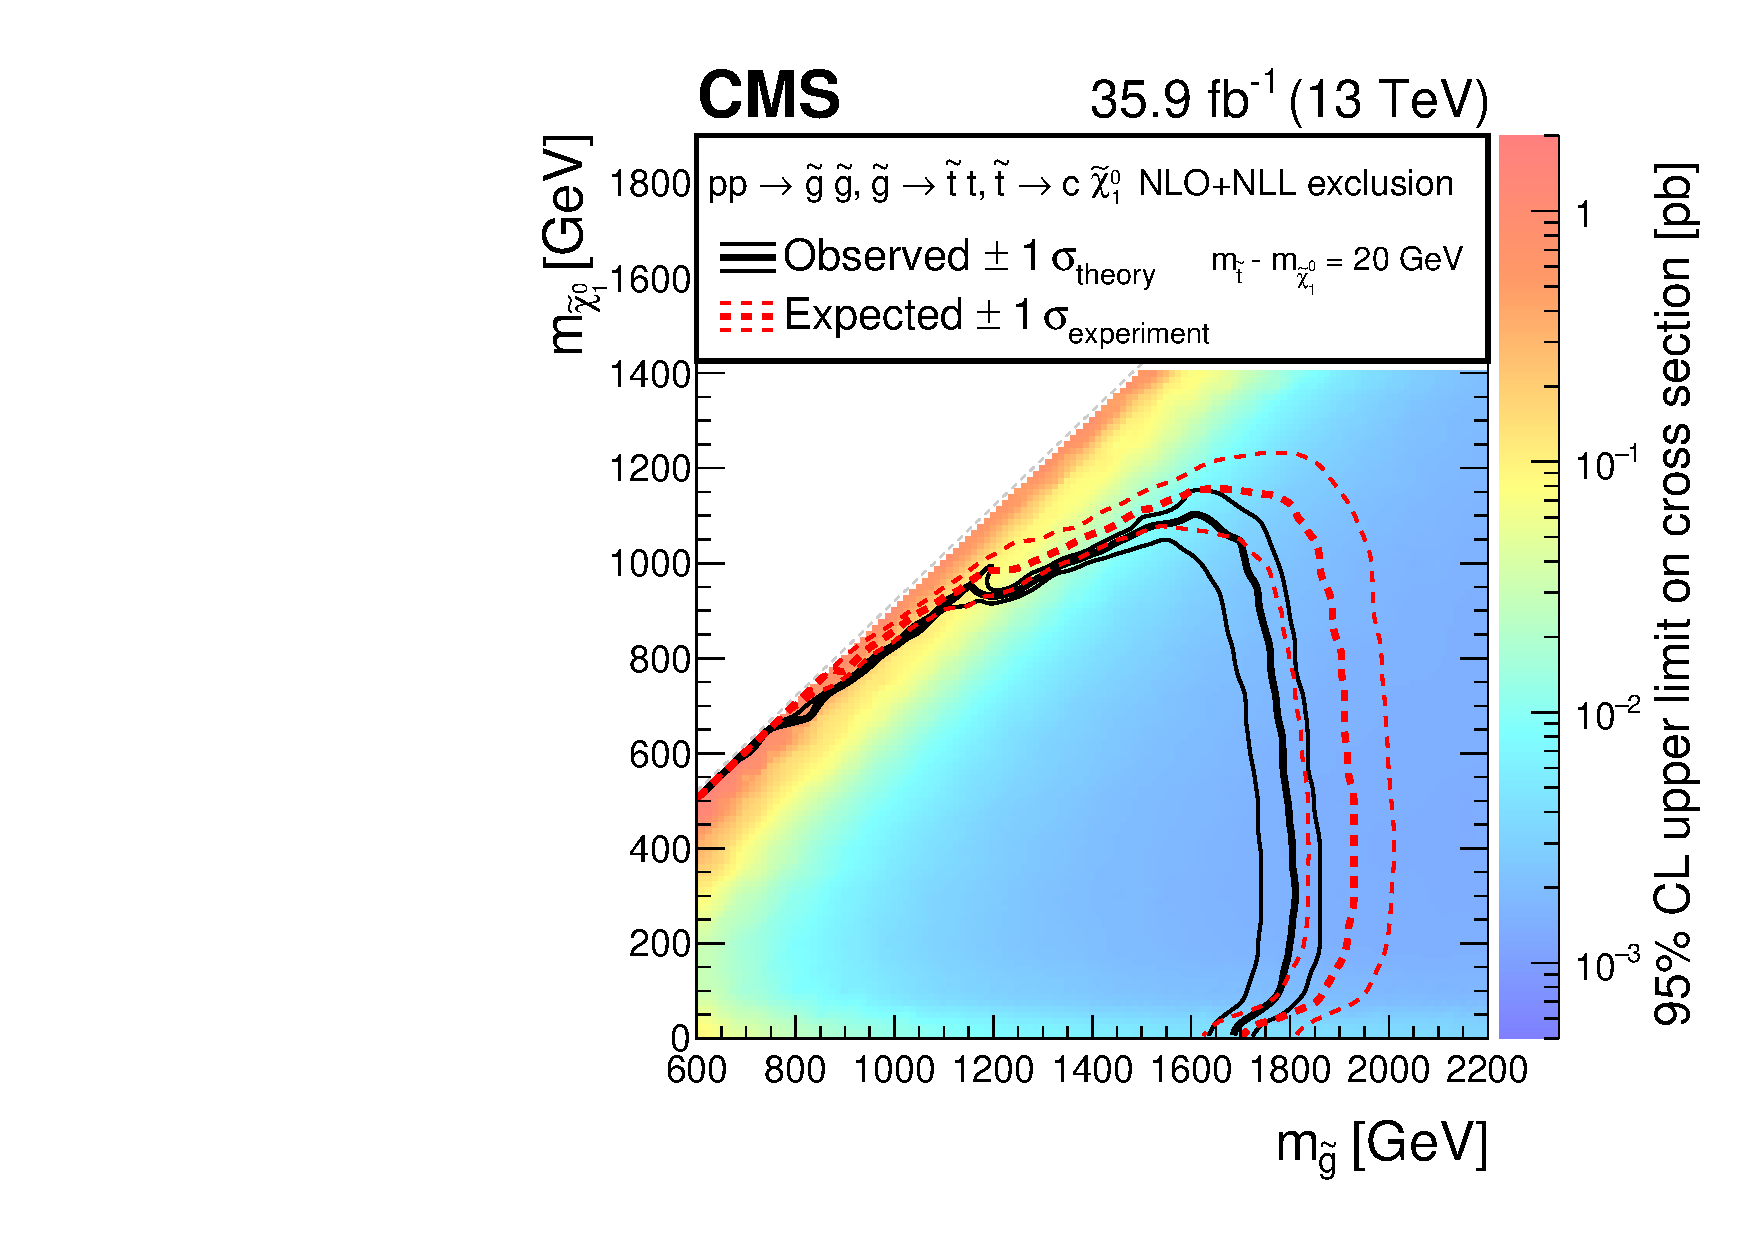
\includegraphics[width=0.40\textwidth]{sections/mc4/Results/figures/T5ttcc_OnlyXSEC.pdf}\\
  \caption{Exclusion limit at 95\% CL for the signal models in this search: top squark pair production with the top squark decaying into a top quark and neutralino (top), and top squarks from cascade decays of gluinos (middle and bottom). The top is T2tt, the middle left model as T1tttt, middle right model as T1ttbb the bottom left one as T5tttt and the bottom right one as T5ttcc.}
  \label{fig:signal_results}
 \end{centering}
\end{figure}

The expected exclusion limits on the model parameters are summarized in Table~\ref{tab:c4limitsummary_exp}:

\begin{table}[htbp]
\fontsize{10 pt}{1.2 em}
\selectfont
\begin{centering}
\caption{\label{tab:c4limitsummary_exp} Expected Exclusion summary table.}
\hspace*{-4ex}
\begin{tabular}{|c|c|c|}
\hline
SMS Model & \specialcell{LSP mass \\ expected exclusion} & \specialcell{SUSY Mother mass \\ expected exclusion} \\
\hline
T2tt & 460 GeV & 1130 GeV \\
\hline
T1tttt & 1100 GeV & 2040 GeV \\
\hline
T1ttbb & 1130 GeV & 1900 GeV \\
\hline
T5tttt & 1080 GeV & 1950 GeV \\
\hline
T5ttcc & 1120 GeV & 1940 GeV \\
\hline
\end{tabular}
\par\end{centering}
\end{table}

The observed exclusion limits on the model parameters are summarized in Table~\ref{tab:c4limitsummary_obs}:

\begin{table}[htbp]
\fontsize{10 pt}{1.2 em}
\selectfont
\begin{centering}
\caption{\label{tab:c4limitsummary_obs} Observed Exclusion summary table.}
\hspace*{-4ex}
\begin{tabular}{|c|c|c|}
\hline
SMS Model & \specialcell{LSP mass \\ observed exclusion} & \specialcell{SUSY Mother mass \\ observed exclusion} \\
\hline
T2tt & 400 GeV & 1020 GeV \\
\hline
T1tttt & 1100 GeV & 2060 GeV \\
\hline
T1ttbb & 1150 GeV & 2000 GeV \\
\hline
T5tttt & 1080 GeV & 2000 GeV \\
\hline
T5ttcc & 1070 GeV & 1850 GeV \\
\hline
\end{tabular}
\par\end{centering}
\end{table}
